\chapter[History of Animal Breeding Methods]{The History of Animal Breeding Methods in the United States}
\label{cha:history-animal-breeding-methods-us}

The first settlers in the New World brought with them such animals as they thought would be most useful. In most cases 
those came from the same communities as the immigrants themselves. Little detail is known about the animals they brought; 
but that is not surprising, since most of the pioneering period was ended in the region east of the Mississippi River 
before the period of herdbooks and pedigree breeding began in Britain. Then, too, during pioneering times the problems of 
defense against marauding men and wild animals and the problems of learning to raise the new crops and of adapting the old 
crops to the new climate overshadowed in importance any question of animal breeding methods.

\index{Making new breeds}Where the new conditions demanded a new type of animal, the pioneers or the first generations of settlers which followed 
them, seem to have been ready to produce that type. Thus, there were developed the Vermont Merino, the cornbelt breeds of 
swine, and horses like the Narragansett pacer, the Conestoga, the Morgan and the Standardbred, the American Saddle Horse, 
the Quarter horse, and many another race of less fame, each of which fitted some local need well enough to become known, 
but many of which never reached the stage of having an organized herdbook. Many of them have ceased to exist, either 
because they were engulfed in the flood of undiscriminating enthusiasm which came later for registered stock or because the 
economic and physical conditions for which they were adapted had ceased to exist. 

It is an interesting but perhaps an idle speculation to wonder whether animal industry in the United States would have been 
more efficient today if in more cases the good local races, already well adapted to local conditions, had been preserved, 
either as pure breeds or as foundations for breeds combining some of the good traits of the local stock and of the imported 
breeds used for improving them. Examples of the latter process are such widely separated cases as the American Saddle Horse 
and Poland-China swine. Allen (\textit{Domestic Animals}, pages 26 and 27), writing in 1847, says of cattle: ``Every 
country and almost every district has its peculiar breeds, which by long association have become adapted to the food and 
circumstances of its position and, when found profitable, they should be exchanged for others, only after the most thorough
trial of superior fitness for the particular location, in those proposed to be introduced.''\index{Adaptation to local conditions}

Appreciation of the usefulness of improved breeding stock followed hard on the heels of the pioneering period. Cattle of 
the Shorthorn, Hereford, and Devon breeds were imported around 1800; although there were yet no herdbooks for those breeds. 
The new pedigree breeding methods of Britain were followed with interest. The individual pedigrees for the Herefords and 
for the Devons in those early importations were not permanently preserved, but some of the pedigrees in the early volumes 
of the American Shorthorn Herdbook trace in part to animals imported as long ago as 1817. Enthusiasm for pedigree breeding
sometimes reached the stage of extreme speculation, as with some of the Merino sheep breeding early in the nineteenth 
century and with the Duchess Shorthorns in the 1870's.

\index{Pedigree breeding, beginnings of}
General interest in pedigree breeding was mainly confined to the Shorthorn breed and to certain light horses and to the 
early sheep breeding in New England until the era of agricultural expansion which began soon after the Civil War. Then 
purebreeding became fashionable for all kinds of animals. The period from 1870 to around 1890 saw the founding and rapid 
expansion of breeding societies for almost all kinds of livestock, each with its herdbook, scorecard, etc. Most of the
breeds were introduced from Britain; although there were a few from other places, such as the Holstein-Friesians from 
Holland and the Brown Swiss from Switzerland and draft horses from Belgium and France. Also, there were some native breeds 
like the cornbelt breeds of swine and the Standardbred and American Saddle Horses. The agricultural colleges, most of which 
were founded just before or early in this period, promoted the movement toward the general use of purebred sires as one of 
the quickest ways to improve the quality and efficiency of animal production. Experiments to find or demonstrate the value 
of the purebred sire in grading up common stock were conducted at some agricultural colleges until well into the 1920's.

The purebreds seemed obviously superior to the common stock in many ways, especially as the country was becoming urbanized 
and the available markets for animals were becoming similar to the markets for which the British stock had been bred for 
many animal generations. The initial gulf betwen the purebreds and the native stock was a wide one in most cases, since no 
large group of high grades with which to compare the purebreds had yet been produced. The most urgent need of the times in 
animal breeding seemed clearly to be a wider use of purebreds.

\index{Grading|(}
\index{Purebreds, superiority of|(}
This expansion in the use of purebred sires made a generally expanding or rising market for the business of producing 
purebred sires. In turn, that favorable economic situation led to the establishment of still more herds and flocks of 
purebreds. Of course this rapid expansion in numbers of purebreds could not continue forever. For most breeds it came to a 
rather abrupt end with the economic depression which began for most agricultural enterprises about 1920. That economic 
crisis merely hastened the end of the remarkable expansion in purebred numbers which began about 1870. There is still room 
for promotion of the wider use of purebred sires, and doubtless some expansion in the total number of purebreds will yet be 
seen; but it will be at a slower percentage rate than was generally true for the half century ending in 1920. There are 
almost enough purebred flocks and herds to produce as many purebred sires as can be sold at a profitable price for use in 
commercial flocks and herds.

This end to the long period of expansion in numbers has meant a serious readjustment of the business of those who produce 
purebreds, and it has also had an effect on the way they regard current breeding problems. There may be nearly enough 
registered sires to supply all the demand which exists or can be aroused by good salesmanship, but there are not enough 
highly meritorious registered sires. Much of the emphasis which used to be given to breed expansion is being changed to breed
improvement.

A contributory cause to this change of emphasis is that for most breeds large numbers of high grades have already been 
produced. Some of those are individually more meritorious in a practical way than the average of the purebreds, even though 
the average of the grades remains below that of the purebreds. Most of the experiments with the use of purebred sires for 
grading have shown that the averages of grades with more than two crosses of pure blood (that is, with more than 75 per
cent pure blood) are very little below the average of the pure breed concerned. When there were no high grades for 
comparison, the differences between different purebreds seemed small and not worth much emphasis, compared with the gulf 
which often existed between the introduced purebred and the common native stock. Now the differences between members of the 
same pure breed are often large compared with the small average differences between purebred and high grade.
\index{Grading|)}

The idea of breed improvement is not new in kind --- it is merely receiving more emphasis than formerly. Nearly all of the \index{Breed associations}
breed associations included improvement of the breed in their very first statements of the objectives of their association. 
An excellent example of that was the insistence by many of the early Holstein-Friesian breeders on the adoption of a system 
of official testing of production before they would merge their two breed associations, one of which lacked this feature.
Nearly every breed association, very early in its existence, adopted a scorecard or some other form of official description 
of the ideal toward which they were working. Occasionally they even went to considerable trouble or expense trying out 
plans which were intended to improve the breed more rapidly. Often these did not work as expected and had later to be 
discarded. Examples are the bounties which the Holstein-Friesian association offered in 1889--1891 for butchering or 
castrating bull calves which would have been eligible for registry, and the ruling of the Hereford association (in effect 
during 1895--1897) that 10 per cent of all applications for registry of bulls would be refused. The Aberdeen-Angus 
Association in 1887 had a rule that of every ten bull calves eligible to registry, one must be castrated or two shall be 
dropped from record. Actually it appears that 70 were castrated and 8 were unrecorded while this was in force.

\begin{figure}[htbp]
    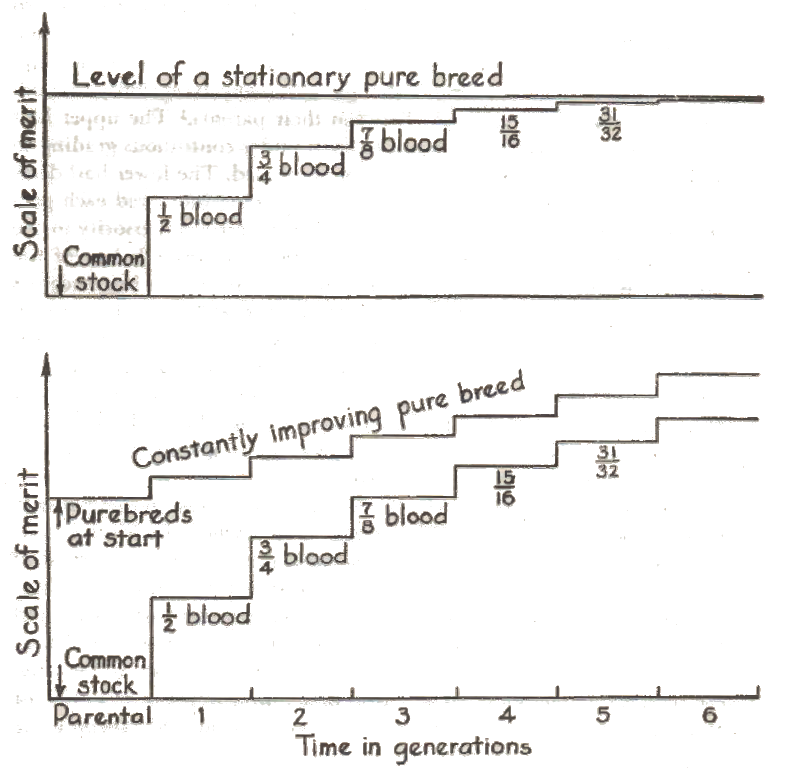
\includegraphics[width=\textwidth]{Figure_2.png}
    \caption{The contrast between grading to a pure breed which is stationary in merit and grading to a pure breed which is improving its merit by a constant amount each generation.}
    \label{fig:Lush_Figure_2}
\end{figure}

The very fact that the purebred has generally been found useful in \index{Grading}grading up common stock carries with it the necessity 
for the continued improvement of the purebred itself if the distinction between pure breds and grades is to be maintained. 
If the pure breed did not continue to improve, the average merit of the grades would soon be so nearly equal to that of the 
purebreds that the distinction between them could not long be maintained. Figure~\ref{fig:Lush_Figure_2} illustrates this on the assumption
(which is true in general, although with many exceptions) that offspring average about half way between their
parents.\footnote{Allowance for regression toward the mean of the groups from which the parents were chosen needs to be 
made if the parents were selected individuals. Also \index{Heterosis}\textit{heterosis} sometimes causes the first-cross generation to be 
better than the diagram indicates.} The upper half of the diagram shows what would happen under continuous grading to a 
pure breed which was not itself being improved. The lower half deals in a similar way with a pure breed which is being 
improved each generation by an amount equal to one-tenth of its initial superiority to the common stock. The difference 
betwen upper and lower halves of the diagram is not important in the first generation or two but becomes 
pronounced after several generations of grading and shows how a continuously improving breed may maintain a commercially 
important margin of superiority over its grades as long as it can continue its own improvement. The diagram, of course, is 
simpler than the facts (as will be seen in more detail in the chapters on selection); but it demonstrates the necessity of 
continued breed improvement to maintain the superiority and popularity of the purebred sire.
\index{Purebreds, superiority of|)}

\index{Making new breeds|(}
Animal breeding history in the United States may be divided into four periods. First, there was a pioneer period when the 
kind of livestock was not of much importance. \index{Making new breeds}Second, there followed a period of developing local races and a little 
experimenting with introduced breeds. Third, came a period of extensive experiments with introduced breeds and widespread 
expansion of organized pure breeding characterized by rivalry between breeds and by breed promotion. In the present period 
the dominant interest is in breed improvement, not only for successful competition with the other breeds, but also for 
keeping the purebreds distinctly ahead of the grades of the same breed in order to maintain a steady demand for purebred 
sires. These periods did not begin and end suddenly but merged gradually into each other, and some of the elements which 
characterize each period were present in lesser degree in all periods. At present it seems likely that plans for
breed improvement will go on within the framework of the existing systems of purebreeding, but here and there occurs some 
experimenting with the combination of more or less blood from two or more breeds, just as was done by some of the breed 
founders in the days before strictly pure breeding and registration became the standard methods of improved breeding.
\index{Making new breeds|)}